\documentclass[11pt]{article}
\usepackage[margin=0.9in]{geometry}
\usepackage{amsmath,amssymb}
\usepackage{booktabs}
\usepackage{graphicx}
\usepackage{caption}
\usepackage[hidelinks]{hyperref}
\captionsetup{font=small,labelfont=bf,skip=6pt}
\setlength{\parskip}{5pt}
\setlength{\parindent}{0pt}
\pagestyle{empty}
\emergencystretch=1.5em

\begin{document}

\begin{center}
{\large\bfseries R-Value: Pricing NBA Production Against True Team Expenditure}
\end{center}
\vspace{2pt}

\textbf{Introduction.} While public player-value metrics assess production, they
fail to take into account the costs involved. The nominal salary greatly
underestimates these costs since, under the luxury tax, a dollar paid by a
repeater taxpayer can cost the franchise several times what a dollar paid by a
team below the limit costs. We want to know which players and teams achieve the
highest level of production for each dollar of true expenditure and whether
cost-efficiency is linked to winning championships. This is a timely question
because the apron system introduced in the 2023 CBA was specifically designed to
limit high-spending rosters.

\textbf{Methods.} The R-Value matches a performance core with a CBA-correct cost
model. The core combines five z-scored components---box production (in terms of
rate and volume), usage-scaled shooting efficiency, minute-shrunk on-court
offensive and defensive impact, and PIE---into a single composite index,
transforms this index using the normal cumulative distribution function into a
score ranging from 0 to 100, and then adjusts it for availability. The weights
assigned to the pillars are determined by a two-stage simplex grid search which
aims to maximise both All-NBA recall@15 and team-win rank correlation. The cost
model calculates the luxury tax for each season based on the bracket schedule
then in effect (from the 2017 CBA through to the 2022--23 season, and thereafter
under the 2023 CBA), applies the repeater rates, and increases each salary by the
team's total-expenditure multiplier. The player R-Value is calculated by dividing
the availability-weighted production by a dampened cost share, while the team
R-Value is obtained by dividing the minute-weighted production by the total
expenditure. The data includes six seasons---2018--19 and the years 2021--22
through 2025--26---excluding the 2019--20 and 2020--21 seasons, which were
disrupted by COVID, since the irregular schedules and the pro-rated tax
settlements in those years compromise the availability and cost models
respectively.

\textbf{Results.} The results show that, using a leave-one-season-out
cross-validation method---where each parameter is refitted excluding the season
for which the performance is being assessed---the performance core recovers
78.9\% of the All-NBA selections among its top 15, as compared to 71.1\% for
PIE$\times$minutes, 34.4\% for raw plus-minus and 23.3\% for estimated net
rating, and that it correlates with team wins at a correlation coefficient of
$\rho = 0.914$ (Table 1). The weights are stable in that four of the six folds
choose the same vector and the offensive-impact weight is the same in all six.

Championships are not usually acquired in an efficient manner (Figure 1). For the
six champions in question, production-per-dollar came in at 16th, 29th, 14th,
13th, 3rd and 14th out of a total of 30. The 2021--22 Warriors secured their
title with an R-Value of 49 compared to a league average of 100, their payroll
being \$179 million and exposing them to a \$191 million repeater tax. A title
score that has been fitted shows that the quality of the eight-man rotation is
about nine times that of the premium associated with the top two stars, and the
actual champions end up ranked 2.83rd out of 30 when assessed against the sample.
Analysis of R-Value on the 2025--26 season's 582 players showed a right skew of
$+1.04$, indicating that there are more overpriced NBA contracts than there
should be.

\textbf{Conclusion.} Cost-efficiency and the prospect of making the playoffs are
almost entirely independent of each other since teams achieve playoff status by
spending during the brief value periods, and the most cost-efficient rosters are
generally two years away from becoming competitive rather than being competitive
now. R-Value expresses that trade-off in terms of CBA-accurate dollars, enabling
front offices to evaluate roster decisions in relation to actual expenditures
rather than just nominal salaries, and it allows players to be ranked, teams to
be assessed and seasons to be forecasted all on the basis of a single model.

\vspace{4pt}
{\small Code and data: \texttt{[GitHub repository]}}

\begin{figure}[h]
\centering
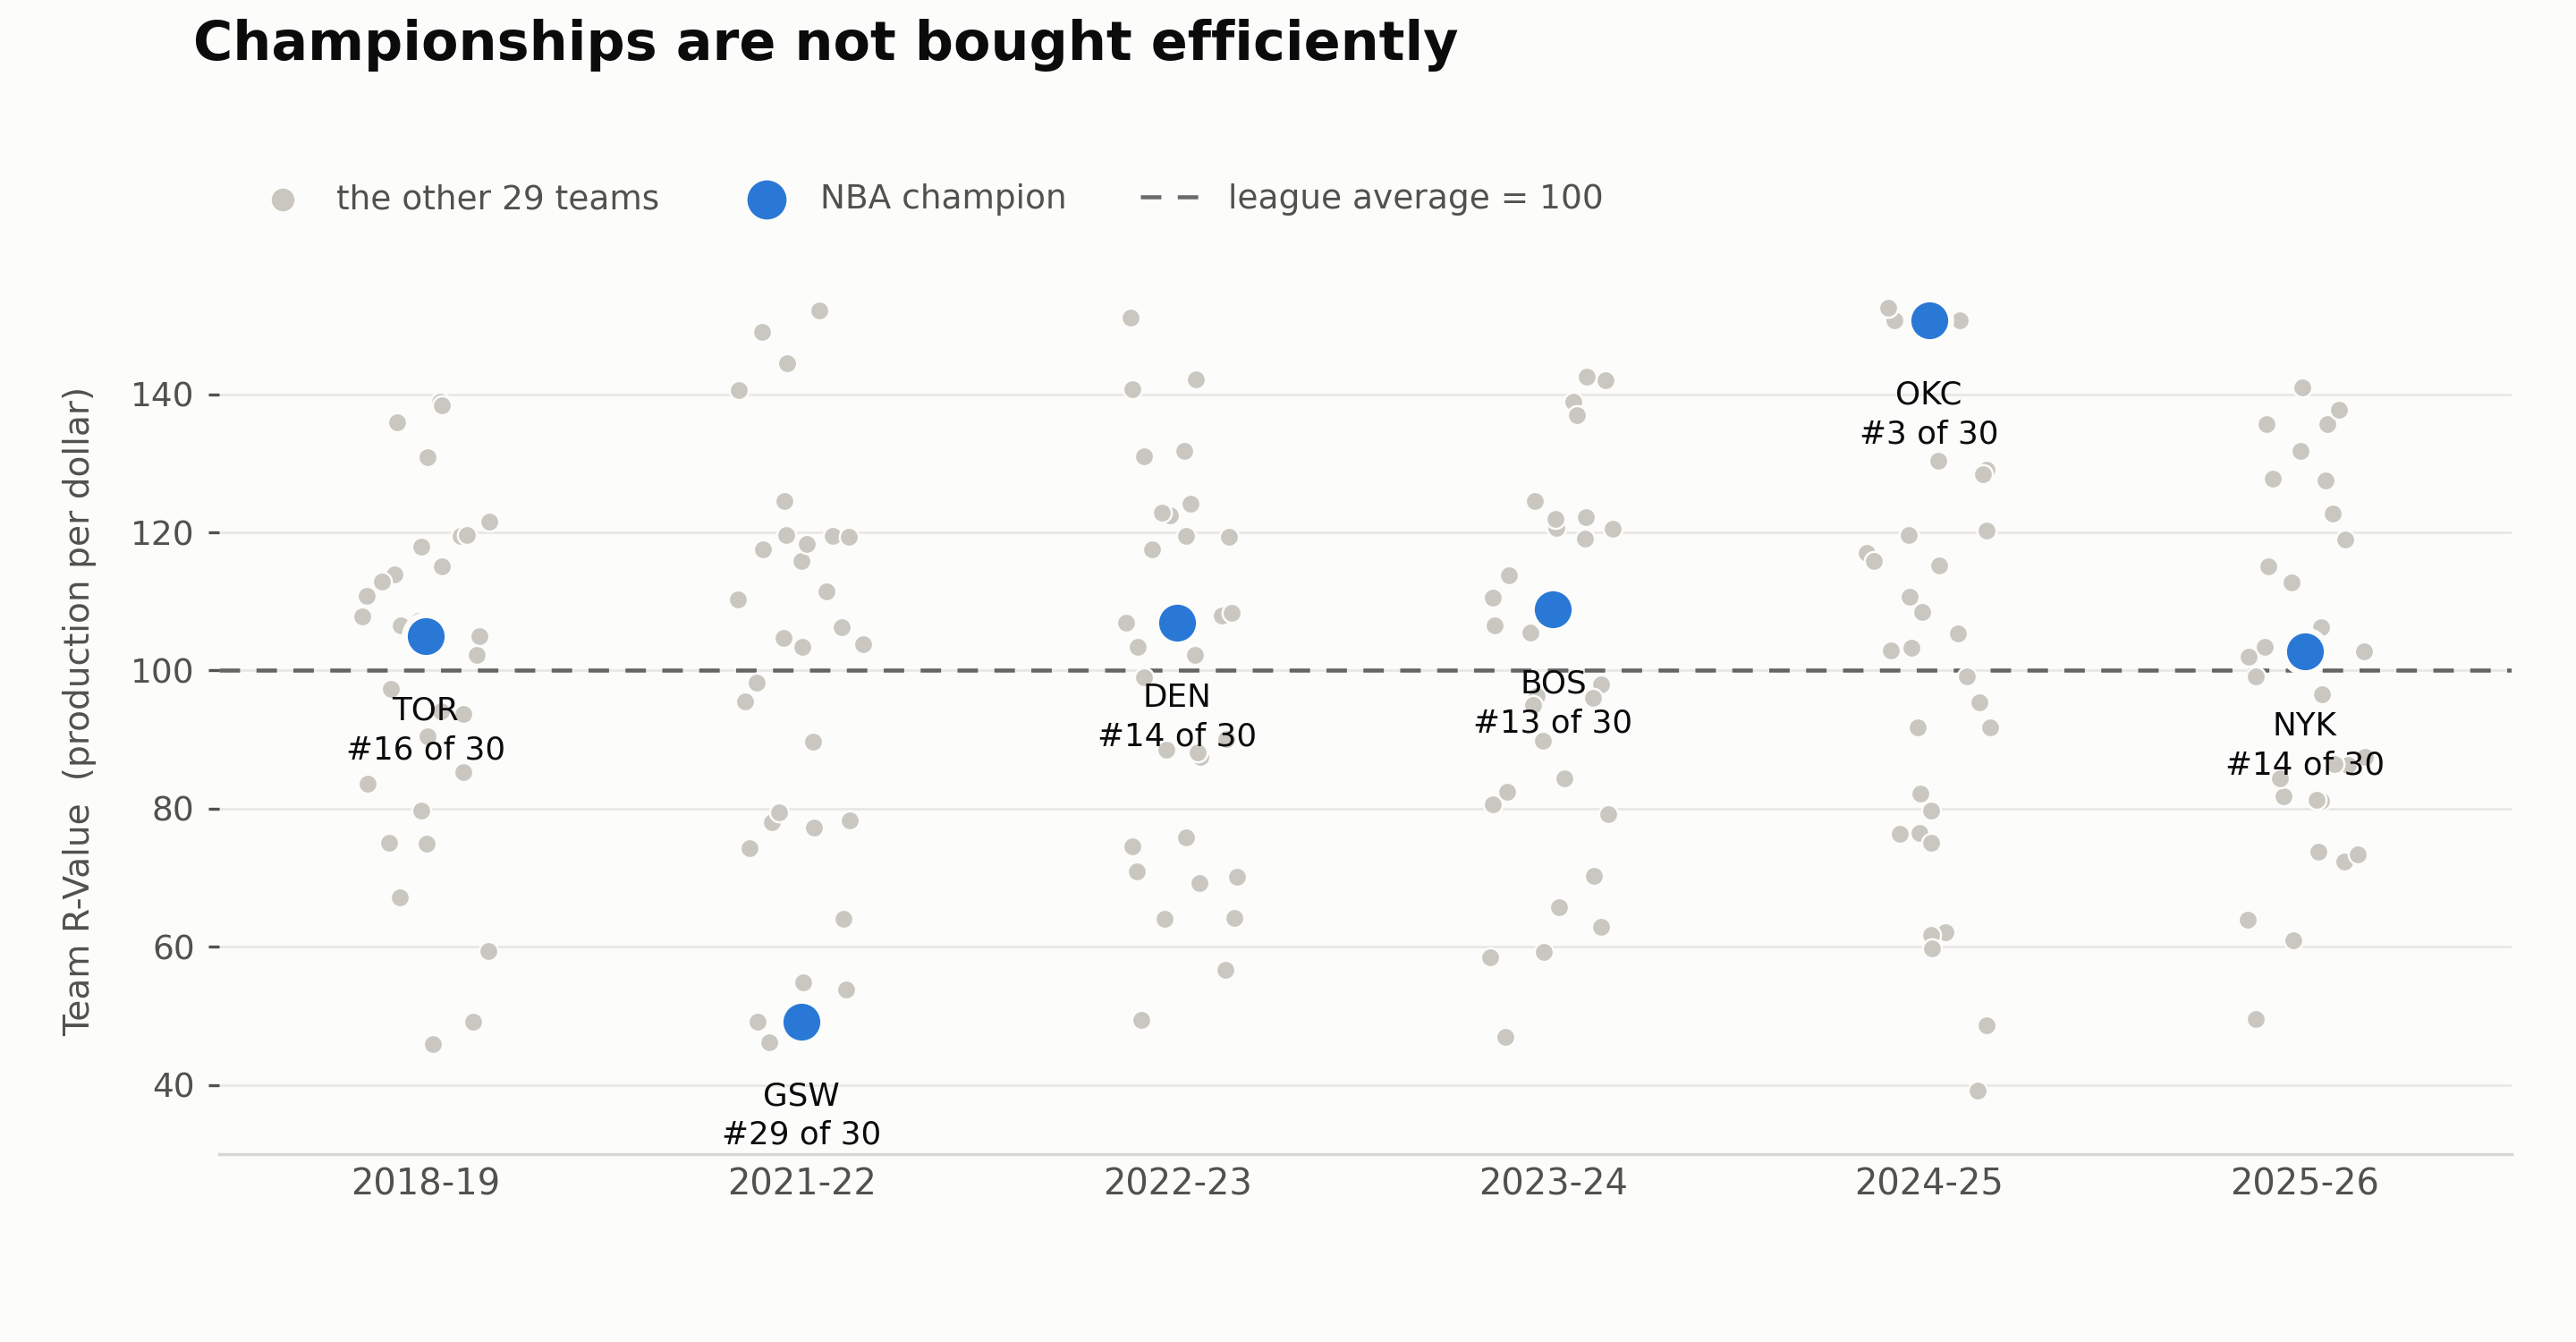
\includegraphics[width=\textwidth]{figure1_champions_value.png}
\caption{Team R-Value for all 30 teams across six seasons, champion highlighted.
Five of the six champions sit at or below the league average of 100.}
\end{figure}

\begin{table}[h]
\centering
\caption{Leave-one-season-out cross-validation. Every parameter (five pillar
weights, two title premiums) is refit on the other five seasons, then scored on
the held-out season.}
\small
\begin{tabular}{lccc}
\toprule
Held-out season & R-Value recall@15 & $\rho$ with wins & Champion title rank \\
\midrule
2018--19 & 0.800 & 0.935 & 1 \\
2021--22 & 0.800 & 0.882 & 3 \\
2022--23 & 0.733 & 0.880 & 6 \\
2023--24 & 0.800 & 0.926 & 1 \\
2024--25 & 0.800 & 0.932 & 3 \\
2025--26 & 0.800 & 0.927 & 3 \\
\midrule
\textbf{Mean (out-of-sample)} & \textbf{0.789} & \textbf{0.914} & \textbf{2.83 of 30} \\
\bottomrule
\end{tabular}

\vspace{5pt}
{\small Benchmarks, which carry no fitted parameters: PIE$\times$minutes 0.711,
raw plus-minus 0.344, estimated net rating 0.233.}
\end{table}

\end{document}
